\setcounter{section}{0}
\section{Introduction}\label{sec:intro}


\vspace{3cm}
\par

\subsection{Life is based on chemical interactions}

Understanding the basis of any biological phenomena is inseparable from understanding the principles that govern the behavior of atoms and molecules. All biological functions depend on events that occur at the molecular level. These events are directed, modulated, or detected by complex biological machines, which are themselves large molecules or clusters of molecules. Included are proteins, nucleic acids, carbohydrates, lipids, and complexes of them. Many areas of biological science focus on the signals detected by these machines or the output from these machines.

Most of biological processes happens in solution, mostly water, with tightly regulated concentrations of ions such as sodium and chloride. These solvent molecules strongly influence the structure and function of molecules, affecting protein folding and stability, as well as the affinity and specificity with which bio-molecules bind.

%As engineers, 
\par








\subsection{Molecular Structure}\label{subsec:molecular_structure}

As we know, molecules are composed of atoms, which are the units of matter that correspond to the elements in the periodic table. For example, only a few of these elements are abundant in cells. In fact, the vast majority of biological matter, about 99\% is made of just six elements: carbon, hydrogen, nitrogen, oxygen, sulfur, and phosphorus \cite{museums1992introduction}. Molecules such as proteins, carbohydrates, lipids, and nucleic acids, are made out of carbon as it's main backbone.\par

Atoms, in turn, are composed of particles known as protons, neutrons, and electrons. The properties of each particle is shown in Table \ref{table:massandcharge}. Protons and neutrons reside in the atomic nucleus and account for almost all of the mass of the atom. The number of protons present in an atom’s nucleus, its atomic number (Z), determines the identity of that atom as an element. 

\par\par

\begin{table}[th] %th for exact position.
    \centering
    \begin{tabular}{l|c|c|c|c}
    \toprule
    Particle            &   Mass [kg]       &   Relative mass [amu] &   Charge [Coulomb]    &   Charge\\
    \midrule
    Proton ($p^{+}$)      &   $1.6726x10^{-27}$ &   1.007                &   $1.6022x10^{-19}$     &   +1\\
    Neutron (n)         &   $1.6749x10^{-27}$ &   1.008                  &   0                   &   0\\
    Electron ($e^{-}$)    &   $9.1094x10^{-31}$ &   $5.489x10^{-4}$       &   $1.6022x10^{-19}$     &   -1\\
    \bottomrule
    \end{tabular}
    \caption{Mass and Charge of individual protons, neutrons and electrons.}
    \label{table:massandcharge}
\end{table}     

\subsubsection{Atomic Structure: Bohr's Model}

Presented by Niels Bohr and Ernest Rutherford in 1913, the Bohr's Model offers a representation of how electrons orbits around the nucleus of an atom. The electron orbits into shells:  The first shell contains 2 electrons, while the next shell can hold 8 electrons. The arrangement of electrons around the atomic nucleus is complex, and electrons do not simply orbit the nucleus as a planet would orbit a star. Broadly speaking, electrons are located in concentric shells that surround the nucleus. The shells that are closer to the nucleus are generally lower in energy than the shells that are farther from the nucleus, meaning that placing an electron in a shell that is closer to the nucleus is more stable and more favorable than placing an electron in a shell that is farther from the nucleus. Because of this, electrons fill shells from the inside to the outside. Electrons in atoms with few electrons are in shells close to the nucleus, whereas atoms with many electrons first utilize the shells that are closer to the nucleus and then those that are farther from the nucleus once the inner shells are filled. 

\subsubsection{Atomic Structure: Quantum Mechanics}

Electrons don't travel in neat 2D circular orbits as the Bohr's model suggest, in fact we can't even determine the position and the velocity of an electron. Instead, we can make predictions about electron's general locations in 3D space. These regions that we call \textbf{orbitals} are the locations in space that has about 90\% certainty that an electron is located somewhere within that region \cite{brown2016introduction}. In Figure \ref{fig:orbitals} are represented the shapes that orbitals can take around the atom. Each orbital now can hold two electrons. In the case of carbon, we focus on the \textit{"s"} orbital, which are spherical in shape with the nucleus of the atom at the center, and \textit{"p"} orbital, which have the shape of the number eight, or the infinity symbol with the nucleus also at the center. 

\begin{figure}[h]
    \centering
    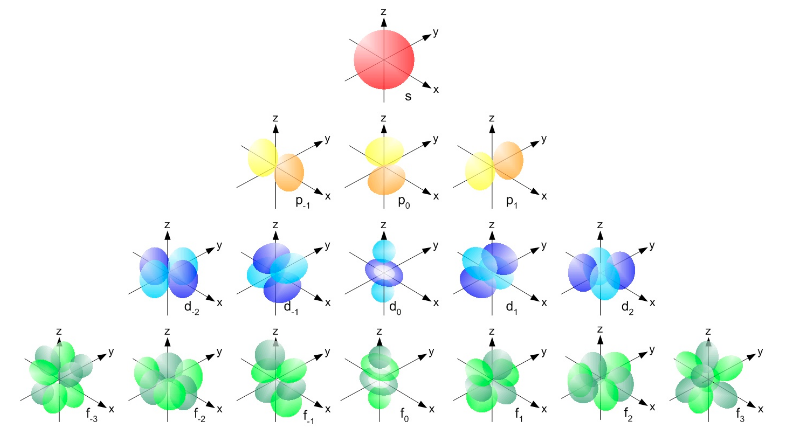
\includegraphics[scale=0.5]{Figures/Chapter1/orbitals.png}
    \caption{Schematics showing the general shapes of s, p, d, and f orbitals.}
    \label{fig:orbitals}
\end{figure}

In the ground state, electrons will occupy the lowest energy orbitals first. In the case of the element \textbf{carbon}, which contains 6 electrons on it's outer shell, the first orbital that fill is the \(1s\), which an hold 2 electrons. Next, is the \(2s\)-orbital which is a larger sphere, and can also hold 2 electrons. Finally, we have \(3p\)-orbital: each one aligned along the \(x,y\) and \(z\)-axis , each capable of 2 electrons so they are filled with one electron in the \(px\)-orbital and one in the \(py\)-orbital. To be stable, carbon wants to fill these three p orbitals with 2 electron each. 

The interaction between different atom's orbitals results in ``connections" between them and can be thinking of forces of attraction (or in some cases repulsion). There are two types of interactions: \textbf{bonded} and \textbf{non-bonded} interactions. The first is know as  chemical bonds, and there are three types: (1) \textit{Ionic bond}, formed when one atom donates valence electrons to another atom. (2) \textit{Covalent bond}, when both atoms share pairs of valence electrons, and (3) \textit{Metallic bond}, formed between a cloud of free electrons and the positively charges ions in a metal. interact. For example, a water molecule is made of one oxygen atom connected to two hydrogen atoms through single covalent bonds.  However, some covalent bonds involve the sharing of more than one pair of electrons between atoms.  Double and triple bonds involve the sharing of four and six valence  electrons,  respectively.   This  versatility  allows  carbon  to  create  many  different kinds of molecules which gives this particular element, a vast number of properties. 

The second interaction, \textbf{non bonded}, is explain in detail in Section \ref{subsec:FF} because is the main objective of this work. Study the behavior of a particular component of this type of interaction. 


\subsection{Computer Simulation of Molecular Systems}\label{subsec:computation}

The role of computation in biology, biological chemistry, and biophysics has shown a steady increase over the past few decades. The continuing growth of computing power (in particular in the context of personal computers) has made it possible to analyze, compare, and characterize large and complex data sets that are obtained from experiments on bio-molecular systems. \cite{van2006biomolecular}. Chemical systems are generally too complex to be treated by analytical theoretical methods so it becomes a necessity to implement numerical analysis to study and predict some properties and configurations.

Computer simulations on models of physical systems have been carried out for more than 65 years now \cite{oostenbrink2007applications}. Many developments have turned molecular dynamics simulations into a valuable tool, complementary to experimental investigation, to probe into structure, dynamics, and activity of large biologically relevant molecules. The thermodynamic information that can be obtained from computer simulations allows analysis and understanding of molecular processes and prediction of molecular properties, highly valued information in medical chemistry and drug design. 




\subsection{Objectives}
\begin{itemize}
    \item The main objective of this work, is to calculate the free energy of solvation (non-polar) of 20 peptides using classical Molecular Dynamics Simulation method.
    \item Compare the results of the explicit MD model with the calculations given by the implicit solvent models available by measure the accuracy of them.
    \item  Become familiar with the use of GROMOS++ software for the calculation of free energies using Thermodynamic Integration. 
    \item Study the behavior of the van der Waals interaction and its contribution to the solvation process. 
    \item Simulate 20 alanine-peptides in a pre-equilibrated water box to preform the free energy calculations. 
\end{itemize}

This document is organized as follow: Section \ref{sec:MD}, presents an overview of the Molecular Dynamics (MD) method, which is the tool to preform the calculations of the free energies of solvation described in the abstract and the criteria and requirements needed to build this method. It also provides a characterization of the force-fields whit a special attention to describe the nature of non-bonded interaction which is the main subject treated in this work.
In Section \ref{sec:implicit}, implicit solvent models are explain with they advantages and disadvantages and also the reasons to use this methods as an alternative to MD. In particular, Section \ref{subsec:CC_method} described a novel way to calculate $\Delta G_{solv}$, sharing the same ideas as the implicit solvent models, but with a clearer physical meaning than current available models. 
Next, Section \ref{sec:Free_energy} presents the underlying thermodynamic and statistical mechanics theory that had been develop to calculate free energies, with the mathematical construction of these models. Section \ref{sec:methods} talks about the methodology used to compute the free energy results, starting with the preparation of the molecular structures (Section \ref{subsec:strucutre_prep}), following by a review of the scope and functionality of GROMOS simulation software, explaining how it was used to preform such calculations step by step. 
Finally, in Section \ref{sec:results} the results and comparison between the models explained above are presented.

